%% The first command in your LaTeX source must be the \documentclass command.
\documentclass[sigconf,authorversion]{acmart}
%% NOTE that a single column version may be required for
%% submission and peer review. This can be done by changing
%% the \doucmentclass[...]{acmart} in this template to
%% \documentclass[manuscript,screen,review]{acmart}

\begin{document}
\settopmatter{printacmref=false}
\setcopyright{none}
\renewcommand\footnotetextcopyrightpermission[1]{}
\pagestyle{plain}
\title{Musical Deep Learning}

%%
%% The "author" command and its associated commands are used to define
%% the authors and their affiliations.
%% Of note is the shared affiliation of the first two authors, and the
%% "authornote" and "authornotemark" commands
%% used to denote shared contribution to the research.
\author{Nhut Minh Phan}
\email{phan92@uw.edu}
\affiliation{%
  \institution{University of Washington}
  \city{Bothell}
  \state{WA}
  \country{USA}
}

\author{Alex Kyllo}
\email{akyllo@uw.edu}
\affiliation{%
  \institution{University of Washington}
  \city{Bothell}
  \state{WA}
  \country{USA}
}

\begin{abstract}
  This paper presents a generative model of multi-instrument symbolic
  music.
\end{abstract}

\keywords{deep learning, neural networks, music}

\maketitle

\section{Introduction}

Machine learning models of music have interesting applications in
music information retrieval and creative tools for musical artists and
educators. Generative models can create accompaniments for music,
transfer styles between clips of music, and even generate entirely new
music. Music is challenging to model because it exhibits a complex
hierarchy of recurring patterns and long-range temporal dependencies,
and because both musical scores and performances have multiple
possible digital representations.

Depending on the task, machine learning models of music may be trained
on the audio signal itself, either in a time domain or a frequency
domain representation, or they may be trained on a digital symbolic
representation of music, the most common of which is MIDI (Musical
Instrument Digital Interface) notation. MIDI is an encoding of music
as streams of bytes in one or more tracks or channels, each
representing a sequence of 128 possible pitch values (where 0 is the
lowest and 127 is the highest), along with timing, pressure and
instrument identifier values. A music transcription model may
transcribe an audio signal as a MIDI score, which can easily be
converted into other symbolic representations such as sheet music for
human performers to read from, while a synthesizer model can convert
MIDI representations into audio signals. A generative music model can
be trained either to generate raw audio, or to produce a symbolic
score that must be played by a synthesizer or by humans to produce an
audio music performance. This project focuses on the latter type of
modeling: generative modeling of symbolic (MIDI) music to compose
original musical scores.

\section{Related Work}

The state of the art in music generation has a long way to go before
it can consistently generate music scores or performances that would
be enjoyable and popular for humans to listen to, but a number of
recent research projects have shown promising progress in this area.

Google's \href{https://magenta.tensorflow.org/}{Magenta} is an
umbrella project for music deep learning research and development of
software tools to expose these models for use by creative artists and
students.

MusicVAE, part of the Magenta project, is a variational Long
Short-Term Memory (LSTM) autoencoder for MIDI that incorporates a
novel hierarchical structure using a ``conductor'' recurrent layer in
its decoder model to better capture structure at multiple levels and
avoid the problem of ``posterior/mode collapse'' whereby a generative
model learns to ignore its latent code and rely on autoregression
\cite{roberts_hierarchical_2018}. This model is trained on 16-bar
paragraphs of music and is capable of generating new melodies that
blend two given melodies via latent space interpolation.

Another Magenta model called Music Transformer is a generative model
that borrows its approach from the Natural Language Processing (NLP)
domain, using a self-attention network to model MIDI music as a
sequence of discrete tokens with relative positional dependencies
\cite{huang_music_2018}. The focus of this model is on learning
long-term dependencies in music to produce longer clips of music with
coherent structure. Music Transformer was trained on a dataset of
Piano-e-competition performances \cite{hawthorne2019enabling} and its
generated piano music received favorable qualitative (Likert scale)
ratings from human listeners for its resemblance to human-composed
music \cite{huang_music_2018}.

MuseGAN \cite{dong2017musegan} is an application of Generative
Adversarial Networks (GAN) to polyphonic MIDI music generation,
trained on four-bar phrases of a multi-track pianoroll representation
of rock songs from the Lakh Midi Dataset
\cite{raffel_learning-based_2016}. Like MusicVAE, MuseGAN includes a
two-level generator that first samples latent codes at the phrase or
bar level, then generates notes within the bars, to produce
longer-term structural patterns.

\begin{figure}[h]
  \centering
  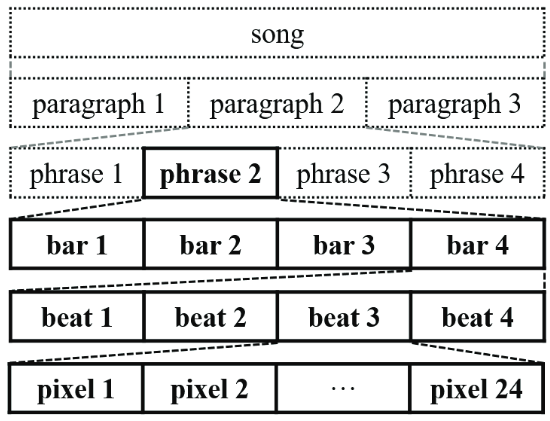
\includegraphics[width=\linewidth]{song_structure.png}
  \caption{Diagram of the hierarchical structure of a musical
    composition, from the MuseGAN paper \cite{dong2017musegan}.}
  \label{song_structure}
  \Description{A diagram showing the hierarchical structure of songs,
    to paragraphs, to phrases, to bars, to, beats, to pixels.}
\end{figure}

A major advantage of working with the symbolic representation of music
is that it is of far lower dimensionality than the raw audio waveforms
of a recorded performance, which makes it less computationally
expensive. However, there are many stylistic aspects of musical
performance that are not captured by a symbolic representation, and
may be specific to a particular performer, so the expressiveness of
symbolic generative models is limited in comparison
\cite{manzelli_conditioning_2018}.

Other research has focused on modeling raw audio waveforms directly. WaveNet is
a causal convolutional neural network for generating raw audio waveforms,
developed by Google DeepMind, which achieves state of the art performance in
generating natural sounding speech from text, but is also capable of generating
short, realistic snippets of audio music \cite{oord_wavenet_2016}.
Another model named SampleRNN generates raw audio waveforms using a three-tier
hierarchy of gated recurrent units (GRU) to model recurrent structure at
multiple temporal resolutions \cite{mehri_samplernn_2017}.

Prior work points out that the division between symbolic music notes
and music performances, is analogous to the division between symbolic
language and utterances in speech, which may inspire ideas for
combining the two approaches \cite{hawthorne2019enabling}. A paper
from Boston University describes an effort to combine the symbolic and
waveform approaches to music modeling, by training an LSTM to learn
melodic structure of different styles of music, then providing
generations from this model as conditioning inputs to a WaveNet-based
raw audio generator \cite{manzelli_conditioning_2018}.

\section{Methods}

\subsection{Datasets}

Two primary datasets will be used for this research project: MusicNet,
which is a collection of 330 freely licensed European classical music
recordings with aligned MIDI scores \cite{thickstun2017learning}, and
the Lakh MIDI Dataset, which includes a collection of 45,129 Creative
Commons licensed MIDI files of popular music songs that have been
matched and aligned to MP3 recordings, and of which I plan to use a
subset for model training and evaluation
\cite{raffel_learning-based_2016}. Including this second dataset may
help to generalize the modeling approach beyond European classical
music to include other popular genres and associated instruments.


\subsection{Data Preprocessing}

Several choices must be made in how to preprocess binary MIDI files
into training examples for a neural network. There are multiple
open-source Python packages that assist with the process of reading
MIDI files from their binary on-disk representations into Python
objects, such as pretty\_midi \cite{raffel_pretty_midi_2014} and
Pypianoroll \cite{dong_pypianoroll_2018}.

In order to accommodate polyphonic music, I will convert each MIDI
file into a pianoroll representation, as visualized in Figure
\ref{pianoroll}, wherein each instrument track is a sparse matrix that
multi-hot encodes the velocity values for each of 128 possible pitch
levels at each timestep. To reduce dimensionality, I will clip the
note pitch values to a narrower range, excluding the rarely used notes
in the extreme high and low octaves, and encode chords (combinations
of notes played simultaneously on the same instrument) as distinct
tokens, so that they can be one-hot encoded

Because songs are typically at least a few minutes long and of varying
length, it will not be feasible to train with entire songs as
examples, so we will crop songs into phrases of equal numbers of
measures to use as training data.

The result of this preprocessing is that each training example will be
a 3D tensor of shape (tracks x ticks x pitches) and stacking the
training examples will produce a 4D tensor.

While we plan to model music with multiple instrument tracks, we
anticipate the need to model only a fixed selection of instrument
parts, similar to how MusicVAE models three-part (drum, bass and
melody) \cite{roberts_hierarchical_2018} and MuseGAN models five-part
(drum, bass, guitar, string, piano) arrangements.

\begin{figure}[h]
  \centering
  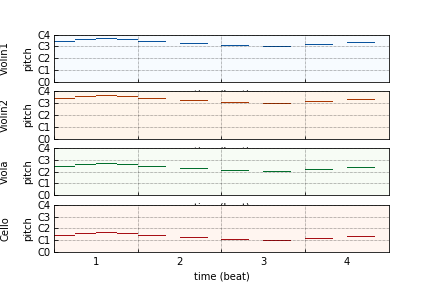
\includegraphics[width=\linewidth]{first_bar.png}
  \caption{Pianoroll visualization of the first measure of
    Beethoven's Serioso String Quartet}
  \label{pianoroll}
  \Description{A pianoroll representation of cello, viola and violin
    parts from a Beethoven piece.}
\end{figure}

Data augmentation is also possible and we assess its impact on
the results--the literature suggests augmentation via pitch shifting
each training example up or down by up to six semitones, and
increasing or reducing the speed by up to 10\% in order to create
additional training examples and reduce overfitting
\cite{oore_this_2018}.

The multi-stream representation discussed in
\cite{kumar2019polyphonic} addresses the issue of extreme class
imbalance and sparsity in the pianoroll representation.

\subsection{Model Design}

\subsection{Model Evaluation}

Evaluation of generative models is challenging because there is no
equivalent of an accuracy metric like what is used in supervised
learning. For autoencoder models we can measure how accurately the
model can reconstruct its own inputs, but this does not tell us the
quality of the interpolated examples. Generative models are typically
evaluated using a combination of qualitative metrics whereby human
judges rate the quality of the generated examples (essentially a
Turing test), and quantitative metrics that assess the differences in
the parametric distributions of generated and real examples. Yang and
Lerch (2020) proposes a set of metrics informed by music theory, for
probabilistically evaluating how similar the generations are to known
sample distributions of real music \cite{yang_evaluation_2020}. These
metrics include counts, ranges, histograms and transition matrices of
pitches and note lengths, then the Kullback-Leibler divergence and
overlapping area of the probability density functions are used to
compare against known reference distributions per musical genre
\cite{yang_evaluation_2020}. Due to the cost and time requirements
associated with designing a human subjects experiment, we
utilize this quantitative approach to the quality assessment of
generated samples.

\section{Results}

\section{Discussion}

\bibliographystyle{ACM-Reference-Format}
\bibliography{paper}

\end{document}
\endinput
